\section{Motor controller}

\subsection{Integration of closed loop}
In order to improve the driving capability of WTR, a closed loop controller has to be integrated in the motor controller. 
This means adding code to integrate two quadrature rotary encoders, adding the controller itself and combining it in a control model.
The control model is explained in the analysis of the current situation section 3.5.

The architecture of the software in the arduino Mega motor controller can be seen in figure \ref{fig::Motorconarc}.

\begin{figure}[H]
\centering
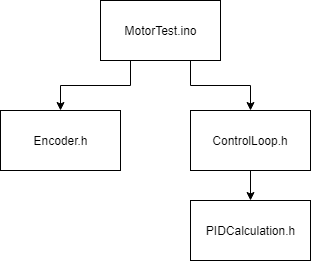
\includegraphics[width=6 cm]{MotorcontrollerArchitecture.png}
\caption{Motorcontroller architecture.}
\label{fig::Motorconarc}
\end{figure}

\subsection{Arduino Mega Code}
The main program combines sends the commands to the actual motor controller via serial bus. 
While one part of the motor controller has been made by the group, a secondary part is a pre-existing part of the original wheelchair WTR is based on.
This is considered a black box, which simply turns the brakes on and off in accordance with the commands sent from the Arduino Mega 2560.
The commands sent to the motor are refreshed at a higher frequency than the control loop is called. %why?
The flow of the main program can be found in figure \ref{fig::MPF}.

\begin{figure}[H]
\centering
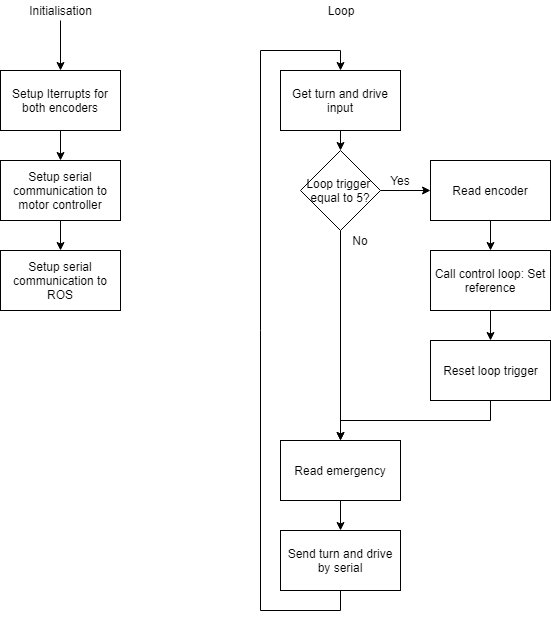
\includegraphics[width=12 cm]{MainProgramFlow.png}
\caption{Main program flow}
\label{fig::MPF}
\end{figure}


\subsection{Rotary encoders}
The rotary encoders are of the quadrature \ref{trm::quad} type with 256 PPR.
Quadrature encoders are equipped with two channels from which one is phase shifted 90 degrees compared to the second, see figure \ref{fig::QuadEnc}.
This allows a program to determine the direction in which the shaft is rotating, as well as the speed; with an increasing resolution 4 times the PPR \ref{trm::PPR}.

\begin{figure}[H]
\centering
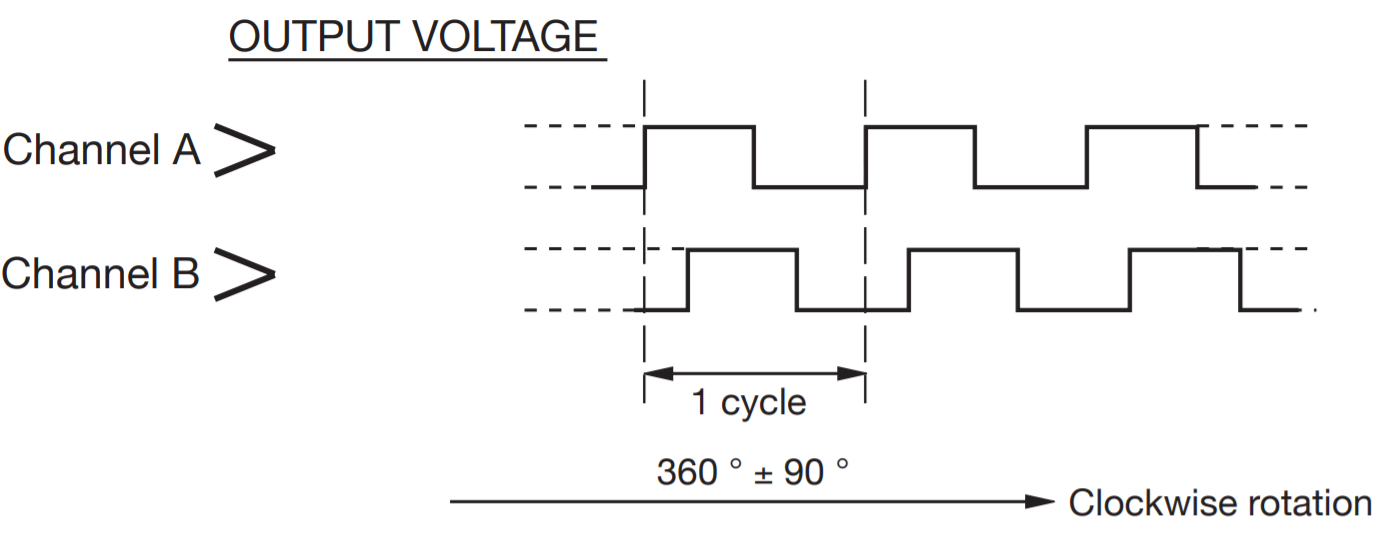
\includegraphics[width=12 cm]{QuadruatureEncoderOutput.png}
\caption{Output from quadrature encoder}
\label{fig::QuadEnc}
\end{figure}

Interrupts are generated for both the rising and falling edge, which increases the resolution to 1024 pulses per revolution.
The speed is determined using code based on the structure which can be found in the the two flowcharts below, \ref{fig::PCF} and \ref{fig::SRC}.
\\
The interrupts will trigger the direction determination function and a speed determination function.
The direction is determined using the logic which can be seen at the left side of figure \ref{fig::PCF}.
The speed is determined by using timers which return the period of the puls, this is converterd to frequency, rad/s and at the end the speed in m/s.
This logic can be found in figure \ref{fig::PCF}.
\\
When the main program wants to know the speed, it will call a speed read function which will then calculate the speed accordingly. Using a read frequency higher then the frequency of the pulses the function will return 0.
This read function can be found in figure \ref{fig::SRC}.

\begin{figure}[H]
\centering
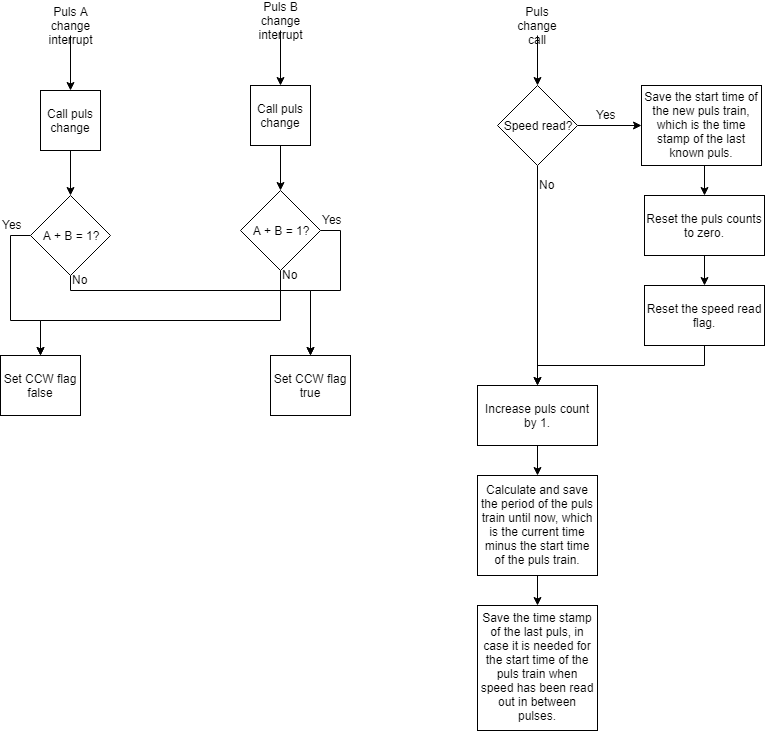
\includegraphics[width=16 cm]{Speed_determinator-Page-1.png}
\caption{Pulse change interrupt flow}
\label{fig::PCF}
\end{figure}


\begin{figure}[H]
\centering
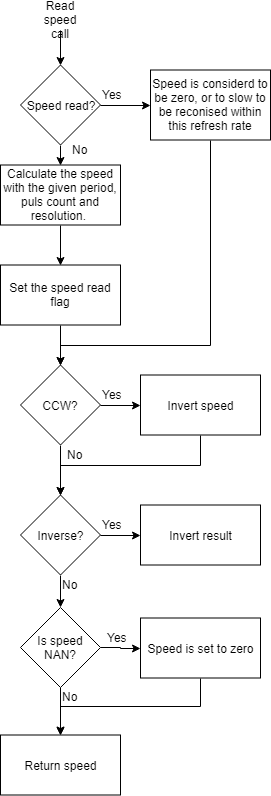
\includegraphics[width=6 cm]{Speed_determinator-Page-2.png}
\caption{Speed read call}
\label{fig::SRC}
\end{figure}

\subsection{Control loop}
The control loop receives an input for both turn and drive. 
Based on the wheel speed received from the encoder class, the turn and drive speed of the robot are calculated. 
Using the inputs and the actual data the turn and drive error are calculated.
The errors are then being send to the turn and drive controllers.
A detailed description of these calculations can be found in movement research. 
The flow of the control loop class can be found in figure \ref{fig::CLF}.

\begin{figure}[H]
\centering
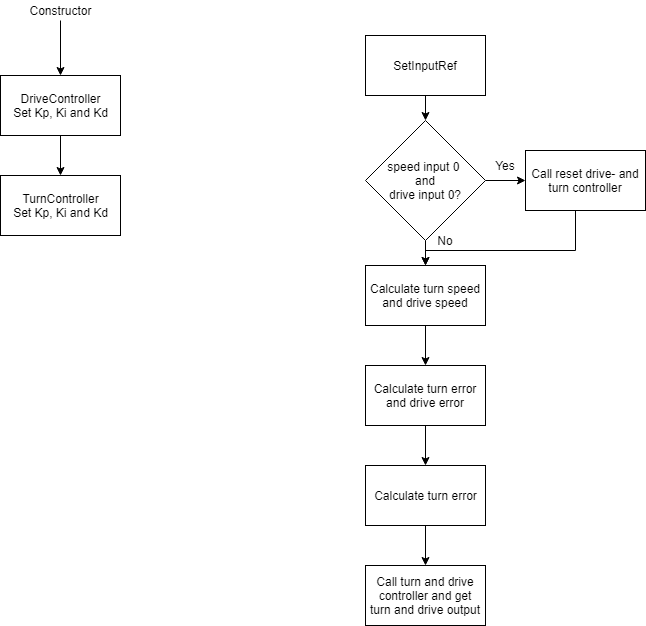
\includegraphics[width=6 cm]{ControlLoop.png}
\caption{Control loop flow}
\label{fig::CLF}
\end{figure}

